\documentclass[11pt,a4paper]{article}

\usepackage[margin=2.3cm]{geometry}
\usepackage[T1]{fontenc}
\usepackage{lmodern}
\usepackage{microtype}
\usepackage{graphicx}
\usepackage{booktabs}
\usepackage{xcolor}
\usepackage{tikz}
\usetikzlibrary{arrows.meta,positioning}
\usepackage{caption}
\usepackage{enumitem}
\usepackage{amsmath}
\usepackage[hidelinks]{hyperref}
\usepackage{float}

\setlist{itemsep=2pt,topsep=4pt}
\captionsetup{font=small,labelfont=bf}
\definecolor{boxblue}{HTML}{E8F1FC}
\definecolor{boxline}{HTML}{2A78D6}

\newcommand{\nQuestions}{64,535}
\newcommand{\nCells}{65}
\newcommand{\nQuestionsRun}{64,478}
\newcommand{\gpuHours}{71}
\newcommand{\nCompared}{29}
\newcommand{\nWithinFive}{12}
\newcommand{\nWithinTen}{20}
\newcommand{\medianAbsDelta}{6.0}
\newcommand{\llamaSCemptyOneK}{25.2}
\newcommand{\llamaSCrtwZero}{205}
\newcommand{\llamaSCwtrZero}{51}
\newcommand{\llamaSCfirstZero}{94.4}
\newcommand{\mistralSCrtwZero}{188}
\newcommand{\mistralSCwtrZero}{29}
\newcommand{\mistralSCfirstZero}{95.6}
\newcommand{\posAccAthree}{60}
\newcommand{\posAccDthree}{43}
\newcommand{\posAccAlong}{42}
\newcommand{\posAccDlong}{23}
\newcommand{\posPickDthree}{14}
\newcommand{\posPickDlong}{8}
\newcommand{\llamaRagRefusalAll}{19.1}

\graphicspath{{figures/}}

\title{\textbf{Improving Long-Context Preference Following in LLMs}\\[2pt]
\large Mid-term Report --- Phase 1: Codebase Setup and Baseline Verification\\
on local open-weight models}
\author{Krishna Jhanwar (12341250)\\ \small\texttt{krishnaj@iitbhilai.ac.in}}
\date{October 2026}

\begin{document}
\maketitle

\begin{abstract}
\noindent
This project builds on PrefEval (Zhao et al., ICLR 2025), a benchmark of 3{,}000 preference--query pairs that measures
whether LLMs keep following a user's stated preference as a conversation grows. The project has three phases: (1)~reproduce
PrefEval's baselines, (2)~train a small preference-detection classifier, and (3)~combine it with a preference memory and a modern
retriever. This report covers Phase~1, which is complete. Because the original evaluation depends on Amazon Bedrock, I rebuilt
the classification-task pipeline to run fully locally on a single RTX~3060 (12\,GB) with Ollama. The original prompt-construction
code is reused verbatim and only the inference call is replaced. Two of the paper's own models were evaluated,
Llama-3-8B-Instruct and Mistral-7B-Instruct-v0.2 (both 8-bit quantized), with all five baseline methods (Zero-shot, Reminder,
Chain-of-Thought, Self-Critic, RAG), for explicit preferences and implicit choice-based preferences, at context lengths from
0.2k to 23k tokens. In total that is \nQuestions{} answered questions in \nCells{} experimental cells (about \gpuHours{} GPU-hours).
Of the \nCompared{} cells that have a published number to compare against (excluding the trivial 0.2k row), \nWithinFive{} are within
5 points of the paper and \nWithinTen{} within 10 (median absolute difference \medianAbsDelta{} points), and the paper's main
qualitative findings reproduce. Along the way I found and fixed three prompt-formatting issues that affect local inference, and two
defects in the released retrieval data. The data also show three behaviours that motivate Phase~3: self-critique frequently
overturns correct answers, accuracy collapses towards an answer-position prior at long context, and retrieved context can
trigger refusals.
\end{abstract}

\tableofcontents
\newpage

%===============================================================================
\section{Project recap and scope of this report}

Large language models deployed as long-running assistants are expected to remember and apply what a user has told them.
PrefEval~\cite{prefeval} shows that they mostly do not. Zero-shot preference-following accuracy falls below 10\% within about
10 turns on its generation task, and even the strongest baselines degrade as unrelated conversation accumulates.
My proposal targets two weaknesses that PrefEval identifies, \emph{long-context retrieval} and \emph{personalization
proactiveness}, in three phases:

\begin{enumerate}[label=\textbf{Phase \arabic*:},leftmargin=5.2em]
  \item \textbf{Codebase setup and baseline verification.} Run the official evaluation and reproduce a slice of the paper's
        classification-task baselines. \emph{Status: complete (this report).}
  \item \textbf{Preference-detection classifier.} Train a small encoder (DistilBERT / ModernBERT / MiniLM) to decide
        whether a conversational turn states a user preference. \emph{Status: design ready (Section~\ref{sec:next}).}
  \item \textbf{Full pipeline.} Classifier $\rightarrow$ structured preference memory $+$ modern retriever (bge / e5),
        evaluated against the Phase~1 baselines. \emph{Status: planned.}
\end{enumerate}

\noindent Phase~1 turned out to be more than ``running the scripts''. The released code calls Amazon Bedrock for every model,
which this project cannot use, and the first local attempt failed with several unrelated errors (Section~\ref{sec:issues}).
I therefore rebuilt the pipeline for local inference, making sure the prompts stay identical to the original and that every run is
resumable and logged. I then ran a much larger grid than the proposal's ``small subset'' so that Phase~3 can be compared
against complete baselines.

%===============================================================================
\section{Background: the PrefEval classification task}

PrefEval contains 1{,}000 preference--query pairs over 20 everyday topics (travel, shopping, lifestyle, entertainment,
education, pets, work). Each pair exists in three \emph{preference forms}:
\begin{itemize}
  \item \textbf{Explicit}: one user sentence, e.g.\ \emph{``I strictly avoid restaurants that serve foods containing gluten
        due to a severe gluten intolerance.''}
  \item \textbf{Implicit, choice-based}: a short dialogue where the assistant offers options and the user's
        acceptance or rejection reveals the preference.
  \item \textbf{Implicit, persona-driven}: a 4--8 turn persona conversation with the preference mentioned in passing
        (not used in Phase~1).
\end{itemize}

The preference is placed at the start of the conversation. Unrelated multi-session turns from LMSYS-Chat-1M~\cite{lmsys}
(\texttt{inter\_turns} user/assistant pairs) follow, and then a query that a generic answer would get wrong
(\emph{``I'll be visiting Rome soon. What are some must-try local restaurants?''}). In the \textbf{classification task} the
model must choose among four options, exactly one of which respects the preference. Accuracy is the share of correct choices,
and the paper averages it over the 20 topics. The five baselines are:
\textbf{Zero-shot}; \textbf{Reminder} (one sentence asking the model to consider earlier preferences);
\textbf{CoT} (five worked examples of preference-aware answers);
\textbf{Self-Critic}~\cite{huang} (answer $\rightarrow$ critique $\rightarrow$ revised answer); and
\textbf{RAG} (top-5 past exchanges retrieved with SimCSE~\cite{simcse} and quoted before the question).

%===============================================================================
\section{Experimental setup}

\subsection{Constraints and model choice}
The paper's models were served through Amazon Bedrock. This project has no Bedrock access, and the compute is one
desktop: NVIDIA RTX~3060 (12\,GB), Intel i7-12700, 15\,GB RAM. I chose \textbf{models that appear in the paper}, so
the reproduced numbers can be compared directly with its Figure~6:

\begin{itemize}
  \item \textbf{Llama-3-8B-Instruct}: Bedrock \texttt{meta.llama3-8b-instruct-v1:0} in the paper;\\
        Ollama \texttt{llama3:8b-instruct-q8\_0} here. Its context window is 8k tokens, so it covers the paper's 0.2k--3k rows only, exactly as
        in the paper.
  \item \textbf{Mistral-7B-Instruct-v0.2}: Bedrock \texttt{mistral.mistral-7b-instruct-v0:2} in the paper;\\
        Ollama \texttt{mistral:7b-instruct-v0.2-q8\_0} here. With a 32k context window it covers the proposal's \emph{long regime} up to 70 turns
        ($\approx$27k tokens).
\end{itemize}
Both models use 8-bit (Q8\_0) weights in Ollama~0.34.0 (llama.cpp backend), with greedy decoding (temperature 0, seed 41).
\textbf{Mixtral-8x7B}, which is also in the paper, was ruled out: its 4-bit build alone is 28.4\,GB, more than the 12\,GB of GPU
memory plus $\approx$10\,GB of free RAM. Smaller 2--3-bit builds would fit only with heavy CPU offload and degraded quality, and would
not be comparable to the paper.

\subsection{Pipeline}
Figure~\ref{fig:pipeline} shows the design. The key decision was \emph{not} to patch the original evaluation scripts but to
vendor the original prompt-building functions unchanged (from upstream commit \texttt{5079505}; only import lines were
edited) and write a new runner around them. The original code builds raw chat-template strings for Llama and Mistral,
which is what Bedrock received. These are sent to Ollama in \emph{raw} mode, so the model sees the same text the authors' models saw.
The answer is parsed with the original \texttt{extract\_choice} function (strict \texttt{<choice>X</choice>} format).
A lenient parse is also stored, as a diagnostic only.

\begin{figure}[H]
\centering
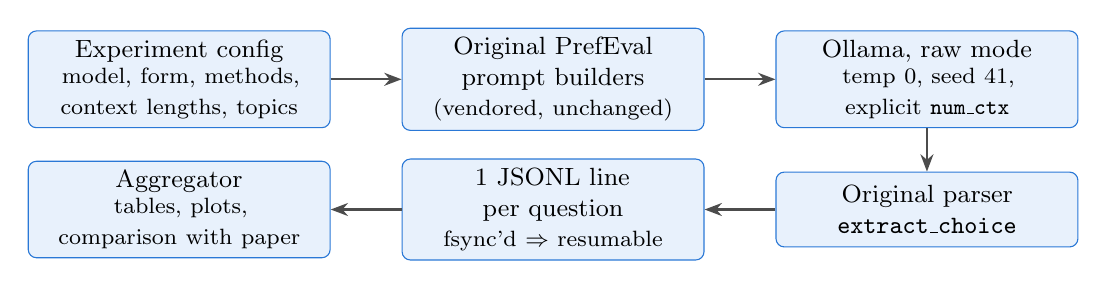
\begin{tikzpicture}[node distance=0.55cm and 0.9cm, font=\small,
  box/.style={draw=boxline, fill=boxblue, rounded corners=3pt, align=center, minimum height=0.95cm, text width=3.6cm},
  arr/.style={-{Stealth[length=2.2mm]}, thick, color=black!70}]
\node[box] (cfg) {Experiment config\\\footnotesize model, form, methods,\\ context lengths, topics};
\node[box, right=of cfg] (up) {Original PrefEval\\prompt builders\\\footnotesize (vendored, unchanged)};
\node[box, right=of up] (oll) {Ollama, raw mode\\\footnotesize temp 0, seed 41,\\ explicit \texttt{num\_ctx}};
\node[box, below=of oll] (parse) {Original parser\\\texttt{extract\_choice}};
\node[box, left=of parse] (res) {1 JSONL line per question\\\footnotesize fsync'd $\Rightarrow$ resumable};
\node[box, left=of res] (agg) {Aggregator\\\footnotesize tables, plots,\\ comparison with paper};
\draw[arr] (cfg) -- (up); \draw[arr] (up) -- (oll); \draw[arr] (oll) -- (parse);
\draw[arr] (parse) -- (res); \draw[arr] (res) -- (agg);
\end{tikzpicture}
\caption{Phase~1 pipeline. Only the inference call differs from the original code. Every run also records its configuration, git
commit, Ollama version, model digest and server settings in a run manifest.}
\label{fig:pipeline}
\end{figure}

\subsection{Context lengths}
The paper labels its rows by approximate prompt size (0.2k, 1k, 3k, \dots). Using the distractor data I confirmed that
these correspond to \texttt{inter\_turns} = 0, 3, 8 (and 28, 48, 68 for the long rows), i.e.\ the paper's ``$N$ turns''
equals \texttt{inter\_turns} + 2. Table~\ref{tab:context} lists the measured prompt sizes. Every model call also records its
prompt length, and \textbf{no prompt was truncated in any run}.

\begin{table}[H]
\centering\small
\begin{tabular}{rrrrr}
\toprule
Paper row & Paper turns & \texttt{inter\_turns} & Llama-3 tokens & Mistral tokens \\
\midrule
0.2k & 2 & 0 & 275 & 309 \\
1k & 5 & 3 & 1,437 & 1,764 \\
3k & 10 & 8 & 3,282 & 4,023 \\
10k & 30 & 28 & -- (8k limit) & 12,139 \\
16k & 50 & 48 & -- (8k limit) & 19,452 \\
23k & 70 & 68 & -- (8k limit) & 26,878 \\
\bottomrule
\end{tabular}

\caption{Mapping between the paper's context rows and \texttt{inter\_turns}, with the measured mean prompt length of
the final zero-shot call (in each model's own tokens; Mistral's tokenizer produces $\approx$10--25\% more tokens).}
\label{tab:context}
\end{table}

\subsection{Experiment grid and compute}
Every cell (model $\times$ form $\times$ method $\times$ context length) was run on \textbf{all 20 topics}. The RAG cells are
the exceptions noted in Section~\ref{sec:issues}. RAG is not defined at 0.2k, because there are no past exchanges to retrieve, and the
paper also reports no value there. Table~\ref{tab:compute} gives the compute. The long-context Mistral runs dominate the cost:
each question processes 12k--28k tokens.

\begin{table}[H]
\centering\small
\begin{tabular}{lrrr}
\toprule
Runs & Questions & GPU hours & s / question \\
\midrule
Llama explicit (Tiers A+B) & 13,751 & 9.0 & 2.3 \\
Llama implicit-choice & 13,901 & 7.6 & 2.0 \\
Mistral explicit, short (Tiers A+B) & 13,853 & 8.6 & 2.2 \\
Mistral explicit, long (10k--23k) & 8,847 & 36.3 & 14.8 \\
Mistral implicit-choice & 13,931 & 9.8 & 2.5 \\
Smoke tests / checks & 195 & 0.1 & 2.7 \\
\midrule
Total & 64,478 & 71.4 & 4.0 \\
\bottomrule
\end{tabular}

\caption{Questions answered and GPU time per group of runs, taken from the run manifest. ``Questions'' counts model
evaluations performed. The final results contain \nQuestions{} questions in \nCells{} complete cells.}
\label{tab:compute}
\end{table}

\paragraph{Engineering for long runs.} Each answered question is appended to its result file and flushed to disk
immediately, so an interrupted run resumes with the same command and loses at most one question. Each result records a
backend revision number, so results from a different prompt-normalisation version can never be mixed in. A guard refuses to
start a run if the Ollama server settings differ from those a model's baselines were produced with
(Section~\ref{sec:issues}), which keeps future Phase~3 comparisons fair.

%===============================================================================
\section{Issues found and how they were resolved}\label{sec:issues}

These issues are part of the result of Phase~1: each would have silently biased the reproduction.

\begin{enumerate}
\item \textbf{The first local attempt failed with several unrelated errors.} The logs showed a top-level Gemini SDK import that fails when
      the package is absent; a missing \texttt{import random} in the original classification script; and three duplicated
      copies of \texttt{generate\_message}, of which only some had been patched for local models (so the self-critic and implicit
      code paths still raised errors). The rewrite avoids all of these by reusing only the pure prompt-building functions.
\item \textbf{Double start-of-sequence token.} The original Llama and Mistral prompts begin with a literal
      \texttt{<|begin\_of\_text|>} / \texttt{<s>}, and Ollama prepends its own. Token counts confirmed the duplication
      (\texttt{"hello"} $\rightarrow$ 3 tokens, \texttt{"<s>hello"} $\rightarrow$ 4 for Mistral). The literal is stripped, so the
      model sees exactly one, as with Bedrock's raw-prompt interface.
\item \textbf{Empty self-critiques (Llama).} The original Llama self-critic templates are indented Python strings and end in
      \texttt{"<|end\_header\_id|>\textbackslash n~~~~~~~~"}. With this trailing whitespace Llama-3 ends its turn immediately,
      producing an empty critique and an empty answer (accuracy near 0). Trimming trailing spaces fixes this. The model
      still sometimes \emph{generates} the indentation and stops, which leaves \llamaSCemptyOneK\% empty revisions for Llama explicit at
      1k (Section~\ref{sec:sc}). Mistral's templates are not indented and are unaffected.
\item \textbf{Silent context truncation.} Ollama truncates prompts longer than its context setting \emph{from the start},
      which is exactly where the preference sits. The context size is therefore set explicitly per model and tier, and every call
      checks the reported prompt length.
\item \textbf{Defects in the released RAG data.} (a) The explicit retrieval file for \texttt{entertain\_games} is
      truncated mid-file in the original repository (only 4/51 questions parse), so explicit RAG is averaged over 19 topics.
      (b) In 7 topics the implicit retrieval files end a few questions early (e.g.\ \texttt{pet\_ownership}: 35 of 43), so
      implicit RAG covers 973 of 1{,}000 questions. The entries that do exist were checked to be aligned with their questions.
      All other methods use all 1{,}000 questions.
\item \textbf{Memory at 32k context.} Mistral with a 32k context did not fit in 12\,GB (10\% of the model ran on the CPU, at 11--695\,s per
      question). Enabling flash attention and an 8-bit KV cache brought it to 100\% GPU at $\approx$2{,}000 tokens/s. Because
      this changes the arithmetic slightly, \emph{all} Mistral runs use this setting and all Llama runs use Ollama's defaults.
      The per-model settings guard enforces this.
\end{enumerate}

%===============================================================================
\section{Results}

\subsection{Explicit preferences: reproduction of the paper's Figure 6}

\begin{figure}[t]
\centering
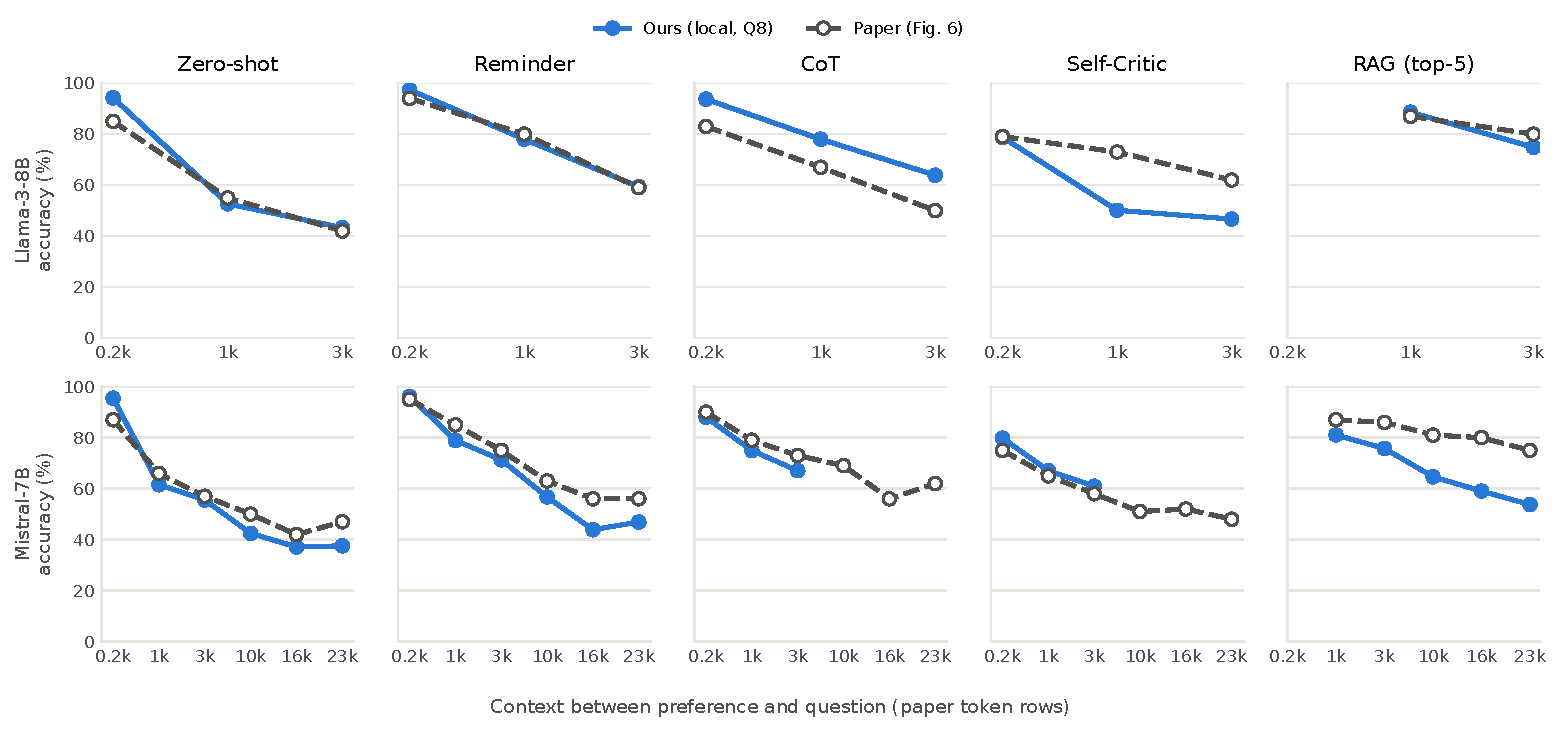
\includegraphics[width=\linewidth]{fig_vs_paper.pdf}
\caption{Classification accuracy on explicit preferences, ours (solid) vs.\ the paper's Figure~6 (dashed), averaged over
20 topics (RAG: 19). Llama-3-8B is limited to 3k tokens by its context window. The paper reports CoT and Self-Critic for
Mistral beyond 3k, which were not run here (Section~\ref{sec:next}).}
\label{fig:vspaper}
\end{figure}

\begin{table}[t]
\centering\small
\textbf{Llama-3-8B-Instruct}\\[2pt]
\begin{tabular}{lrrr}
\toprule
Method & 0.2k (0) & 1k (3) & 3k (8) \\
\midrule
Zero-shot & 94.2 / 85 (+9.2) & 52.7 / 55 ($-$2.3) & 43.3 / 42 (+1.3) \\
Reminder & 97.4 / 94 (+3.4) & 78.0 / 80 ($-$2.0) & 59.4 / 59 (+0.4) \\
CoT & 93.7 / 83 (+10.7) & 78.0 / 67 (+11.0) & 63.9 / 50 (+13.9) \\
Self-Critic & 78.8 / 79 ($-$0.2) & 50.1 / 73 ($-$22.9) & 46.7 / 62 ($-$15.3) \\
RAG (top-5) & -- & 88.6 / 87 (+1.6) & 74.8 / 80 ($-$5.2) \\
\bottomrule
\end{tabular}
\\[8pt]
\textbf{Mistral-7B-Instruct-v0.2}\\[2pt]
\resizebox{\linewidth}{!}{\begin{tabular}{lrrrrrr}
\toprule
Method & 0.2k (0) & 1k (3) & 3k (8) & 10k (28) & 16k (48) & 23k (68) \\
\midrule
Zero-shot & 95.5 / 87 (+8.5) & 61.5 / 66 ($-$4.5) & 55.5 / 57 ($-$1.5) & 42.5 / 50 ($-$7.5) & 37.1 / 42 ($-$4.9) & 37.6 / 47 ($-$9.4) \\
Reminder & 96.2 / 95 (+1.2) & 78.9 / 85 ($-$6.1) & 71.3 / 75 ($-$3.7) & 56.7 / 63 ($-$6.3) & 43.9 / 56 ($-$12.1) & 46.9 / 56 ($-$9.1) \\
CoT & 88.0 / 90 ($-$2.0) & 74.9 / 79 ($-$4.1) & 67.0 / 73 ($-$6.0) & -- & -- & -- \\
Self-Critic & 79.8 / 75 (+4.8) & 67.0 / 65 (+2.0) & 61.0 / 58 (+3.0) & -- & -- & -- \\
RAG (top-5) & -- & 81.0 / 87 ($-$6.0) & 75.7 / 86 ($-$10.3) & 64.6 / 81 ($-$16.4) & 59.0 / 80 ($-$21.0) & 53.7 / 75 ($-$21.3) \\
\bottomrule
\end{tabular}
}
\caption{Explicit preference, classification accuracy (\%): ours / paper (difference). Context columns are the paper's
token rows with \texttt{inter\_turns} in parentheses.}
\label{tab:vspaper}
\end{table}

Figure~\ref{fig:vspaper} and Table~\ref{tab:vspaper} compare all cells with published numbers. Excluding the trivial
0.2k row, \nWithinFive{} of \nCompared{} cells are within 5 points of the paper and \nWithinTen{} within 10 (median absolute
difference \medianAbsDelta{}). The differences are mostly systematic rather than random:

\begin{itemize}
  \item \textbf{Zero-shot and Reminder reproduce closely} for both models up to 3k (e.g.\ Llama Reminder 97.4 / 78.0 / 59.4
        vs.\ 94 / 80 / 59). With no distractors (0.2k), our zero-shot accuracy is 8--9 points \emph{higher} than the paper's for
        both models.
  \item \textbf{CoT differs by model.} It is 11--14 points above the paper for Llama and 2--6 points below for Mistral.
        Prompts and parsing are identical, so this most likely reflects differences in how the models are served (quantization
        and decoding) rather than a systematic pipeline bias.
  \item \textbf{Self-Critic matches for Mistral} (within 2--5 points at all lengths) but is 15--23 points low for Llama at 1k / 3k.
        The difference comes from the original Llama template (issue~3): excluding empty revisions brings Llama to 78.8 / 67.1 /
        47.8.
  \item \textbf{RAG matches for Llama} (88.6 / 74.8 vs.\ 87 / 80) but falls increasingly below the paper for Mistral as context
        grows ($-6$ at 1k to $-21$ at 16k / 23k). Mistral is the model that uses an 8-bit KV cache at long context, and RAG prompts are
        the longest, so quantization error accumulating over long prompts is a plausible explanation. I have \emph{not} yet verified it
        with a full-precision control run.
\end{itemize}

\subsection{Long context (Mistral-7B, up to 23k tokens)}

\begin{figure}[t]
\centering
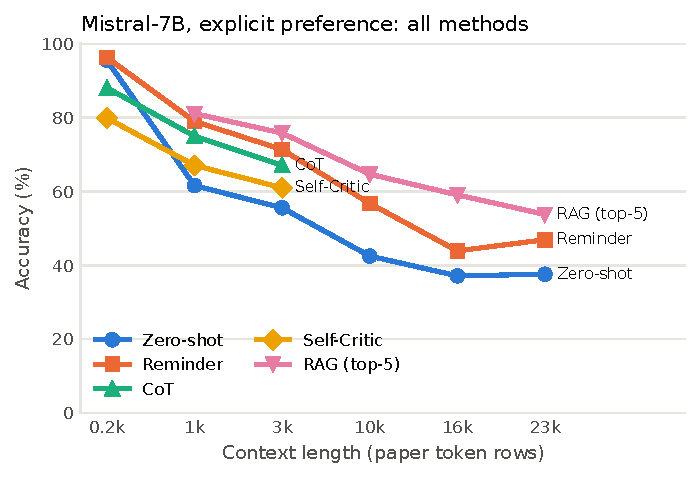
\includegraphics[width=0.66\linewidth]{fig_mistral_long.pdf}
\caption{All methods for Mistral-7B on explicit preferences. CoT and Self-Critic were run up to 3k.}
\label{fig:long}
\end{figure}

Figure~\ref{fig:long} reproduces the paper's qualitative picture. Accuracy falls steeply between 0.2k and 10k and then
flattens. Reminder stays above Zero-shot at every length, and RAG is the best method throughout (53.7\% at 23k vs.\ 37.6\% for
Zero-shot). A lesson from the run order: the first long-context pilot used three topics, and on those Zero-shot reached only
$\approx$23\% at 23k, essentially chance. Those three topics turned out to be among the hardest in the benchmark
(Figure~\ref{fig:heatmap}). Over all 20 topics the value is 37.6\%. Topic choice changes the conclusions substantially, which is why
all reported numbers use the full 20 topics.

\subsection{Implicit (choice-based) preferences}

The paper reports implicit preferences only for the \emph{generation} task (its Tables 8--13), which needs a Claude-3-Sonnet
judge. The classification numbers below are therefore new baselines, not reproductions. They are the reference for Phase~3,
which the proposal scopes to explicit and implicit-choice preferences.

\begin{table}[H]
\centering\small
\begin{tabular}{l rrr rrr}
\toprule
 & \multicolumn{3}{c}{Llama-3-8B} & \multicolumn{3}{c}{Mistral-7B} \\
\cmidrule(lr){2-4}\cmidrule(lr){5-7}
Method & 0.2k & 1k & 3k & 0.2k & 1k & 3k \\
\midrule
Zero-shot & 77.0 & 53.3 & 46.0 & 81.0 & 50.8 & 47.5 \\
Reminder & 91.0 & 77.0 & 60.2 & 88.4 & 71.9 & 63.1 \\
CoT & 84.4 & 70.3 & 61.7 & 74.0 & 60.1 & 59.5 \\
Self-Critic & 66.1 & 50.1 & 38.7 & 67.2 & 51.8 & 50.9 \\
RAG (top-5) & -- & 82.8 & 73.7 & -- & 69.0 & 64.0 \\
\bottomrule
\end{tabular}

\caption{Implicit choice-based preferences, classification accuracy (\%), 20 topics (RAG: 973 of 1{,}000 questions).}
\label{tab:implicit}
\end{table}

\begin{figure}[H]
\centering
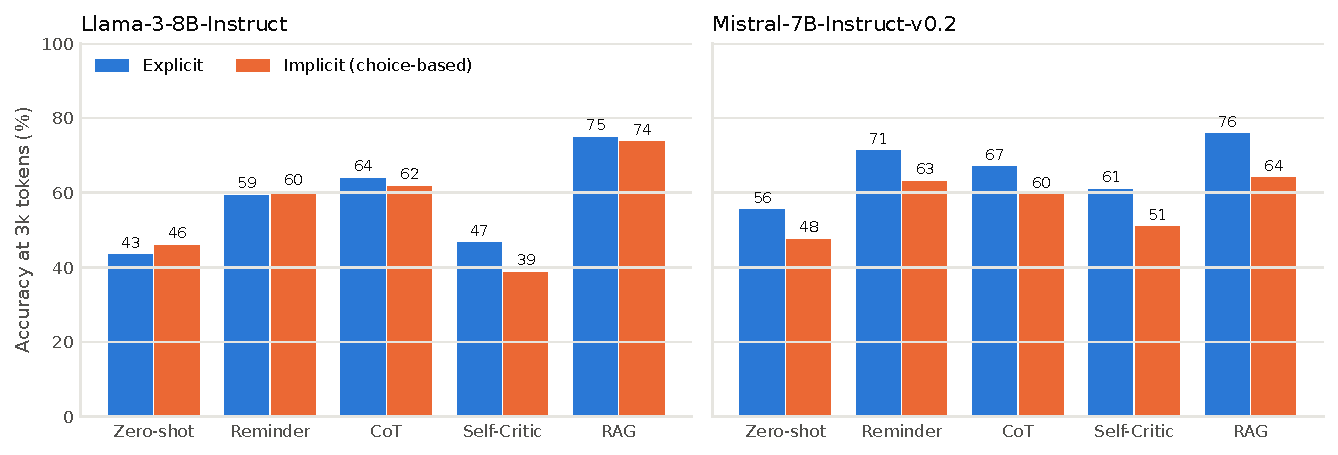
\includegraphics[width=0.92\linewidth]{fig_explicit_vs_implicit.pdf}
\caption{Explicit vs.\ implicit (choice-based) preferences at 3k tokens.}
\label{fig:expimp}
\end{figure}

Implicit preferences are harder, as the paper finds for generation, but the two models differ (Figure~\ref{fig:expimp}).
\textbf{Mistral} is 7--15 points worse on implicit preferences for every method at every length. \textbf{Llama} loses accuracy
mainly when there are no distractors (Zero-shot 77.0 vs.\ 94.2 at 0.2k). At 3k its explicit and implicit scores are within
3 points for Zero-shot, Reminder, CoT and RAG. This suggests that \emph{locating} the preference becomes the bottleneck as context grows, more than
how it was expressed. Self-Critic is the exception: it is 8 points worse on implicit preferences at 3k. Among the prompting methods, Reminder
and CoT both improve substantially over Zero-shot on implicit preferences once distractors are present (CoT: +9 to +17 points), with
Reminder as good as or better than CoT. RAG is the best method for Llama.

\subsection{Analyses that motivate Phase 3}

\paragraph{Self-critique mostly changes correct answers.}\label{sec:sc}
Table~\ref{tab:sc} and Figure~\ref{fig:sc} compare each question's first answer with its final answer after critique and revision.
With no distractors the first answer is almost always right (Llama \llamaSCfirstZero\%, Mistral \mistralSCfirstZero\%), and the
revision step turns \llamaSCrtwZero{} (Llama) and \mistralSCrtwZero{} (Mistral) correct answers wrong while fixing only
\llamaSCwtrZero{} and \mistralSCwtrZero. At longer contexts the revision changes a large share of answers in both directions, and the net effect
ranges from $-6$ to $+7$ points across models and forms. This matches the paper's observation that iterative self-feedback is less effective for classification. It also motivates
the proposal's approach: preference information should enter the prompt deliberately, rather than relying on the model to rediscover it
through self-reflection.

\begin{figure}[H]
\centering
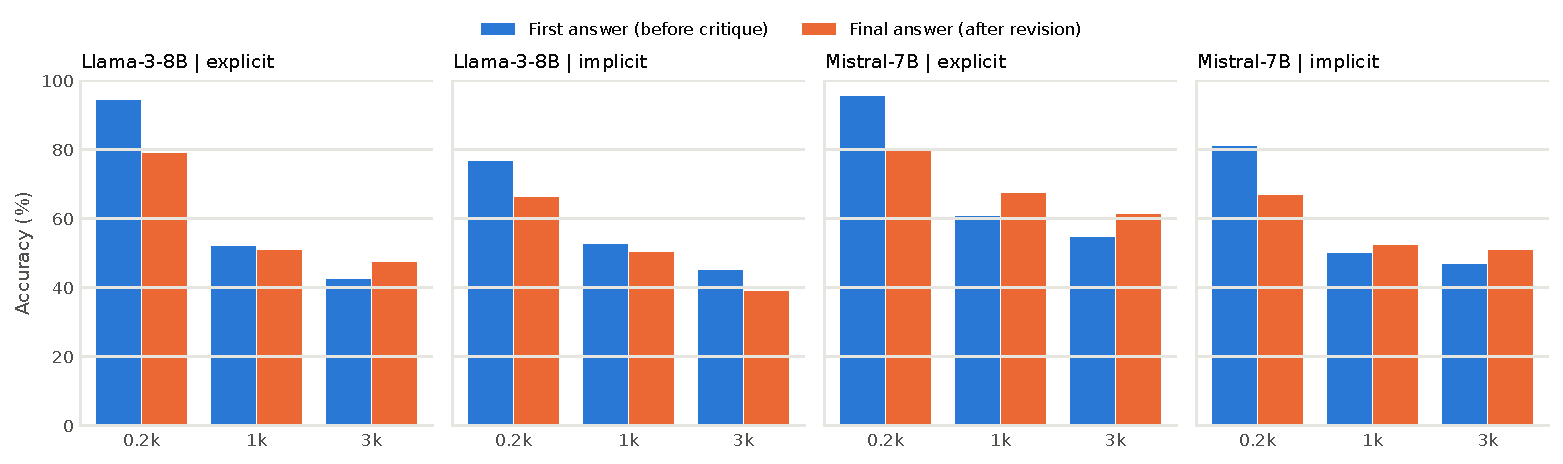
\includegraphics[width=\linewidth]{fig_selfcritic.pdf}
\caption{Self-Critic: accuracy of the first answer vs.\ the final revised answer.}
\label{fig:sc}
\end{figure}

\begin{table}[H]
\centering\small
\begin{tabular}{ll r rrrrr}
\toprule
Model & Form & Context & First & Final & R$\to$W & W$\to$R & Empty (\%) \\
\midrule
Llama-3-8B & explicit & 0.2k & 94.4 & 79.0 & 205 & 51 & 0.0 \\
Llama-3-8B & explicit & 1k & 51.9 & 50.7 & 318 & 306 & 25.2 \\
Llama-3-8B & explicit & 3k & 42.3 & 47.4 & 312 & 363 & 2.5 \\
Llama-3-8B & implicit & 0.2k & 76.5 & 66.2 & 303 & 200 & 0.1 \\
Llama-3-8B & implicit & 1k & 52.4 & 50.3 & 350 & 329 & 1.4 \\
Llama-3-8B & implicit & 3k & 44.9 & 39.0 & 356 & 297 & 0.0 \\
Mistral-7B & explicit & 0.2k & 95.6 & 79.7 & 188 & 29 & 0.2 \\
Mistral-7B & explicit & 1k & 60.7 & 67.4 & 208 & 275 & 0.0 \\
Mistral-7B & explicit & 3k & 54.7 & 61.1 & 207 & 271 & 0.0 \\
Mistral-7B & implicit & 0.2k & 80.9 & 66.7 & 264 & 122 & 0.3 \\
Mistral-7B & implicit & 1k & 49.8 & 52.2 & 277 & 301 & 0.1 \\
Mistral-7B & implicit & 3k & 46.6 & 50.9 & 244 & 287 & 0.0 \\
\bottomrule
\end{tabular}

\caption{Self-Critic details (accuracies pooled over questions). R$\to$W / W$\to$R: questions whose answer changed from
right to wrong / wrong to right. Empty: final answers without any choice (Llama template issue, Section~\ref{sec:issues}).}
\label{tab:sc}
\end{table}

\paragraph{At long context the model falls back on answer position.}
Option order is shuffled per question, so a model that ignores the preference should be right about 25\% of the time regardless
of where the correct option is. Figure~\ref{fig:pos} shows otherwise for Mistral zero-shot. As context grows, accuracy depends more and more on the
\emph{position} of the correct option: it is \posAccAthree\% vs.\ \posAccDthree\% for A vs.\ D at 3k, and \posAccAlong\% vs.\ \posAccDlong\% at
23k. The model increasingly favours option B and avoids option D, which it picks only \posPickDlong\% of the time at 23k (\posPickDthree\% at 3k). Once the
preference is no longer used, what remains is a position prior. This is a concrete failure mode that a preference memory placed
next to the question should counteract.

\begin{figure}[H]
\centering
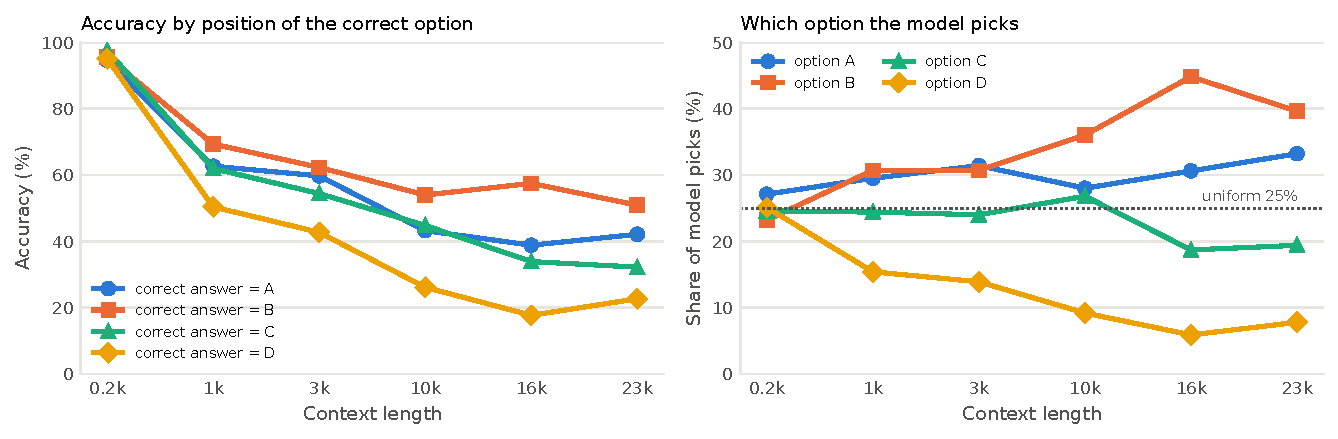
\includegraphics[width=0.92\linewidth]{fig_position_bias.pdf}
\caption{Mistral-7B, explicit zero-shot: accuracy by position of the correct option (left) and distribution of the model's
picks (right).}
\label{fig:pos}
\end{figure}

\paragraph{Retrieved context can trigger refusals.}
For Llama with RAG at 3k, \llamaRagRefusalAll\% of answers contain no valid choice. These are almost all refusals such as
\emph{``I cannot recommend any\dots''}, concentrated in food and travel topics (Figure~\ref{fig:refusal}). The retrieved
snippets include unrelated LMSYS exchanges, and together with a dietary restriction they make the model overly cautious. Mistral
shows this rarely (0.6\%). This supports the proposal's point that retrieved raw exchanges can act as distractors, and that a
filtered, structured preference memory may be the better input.

\begin{figure}[H]
\centering
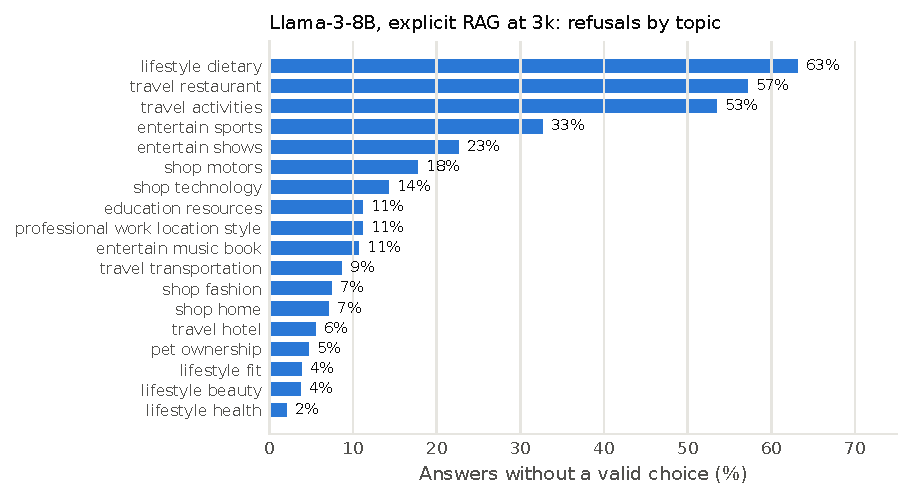
\includegraphics[width=0.62\linewidth]{fig_rag_refusals.pdf}
\caption{Llama-3-8B, explicit RAG at 3k: share of answers without a valid choice, by topic.}
\label{fig:refusal}
\end{figure}

\paragraph{Topic difficulty varies widely.} Figure~\ref{fig:heatmap} breaks the 3k results down by topic. Food and travel topics
(\texttt{lifestyle\_dietary}, \texttt{travel\_restaurant}, \texttt{travel\_activities}) are the hardest on average across methods and both models.
These preferences are often restrictions (allergies, diets), and the generic recommendation violates them.
This heterogeneity is why results on a few topics can mislead, and why Phase~3 must report per-topic results alongside the average.

\begin{figure}[H]
\centering
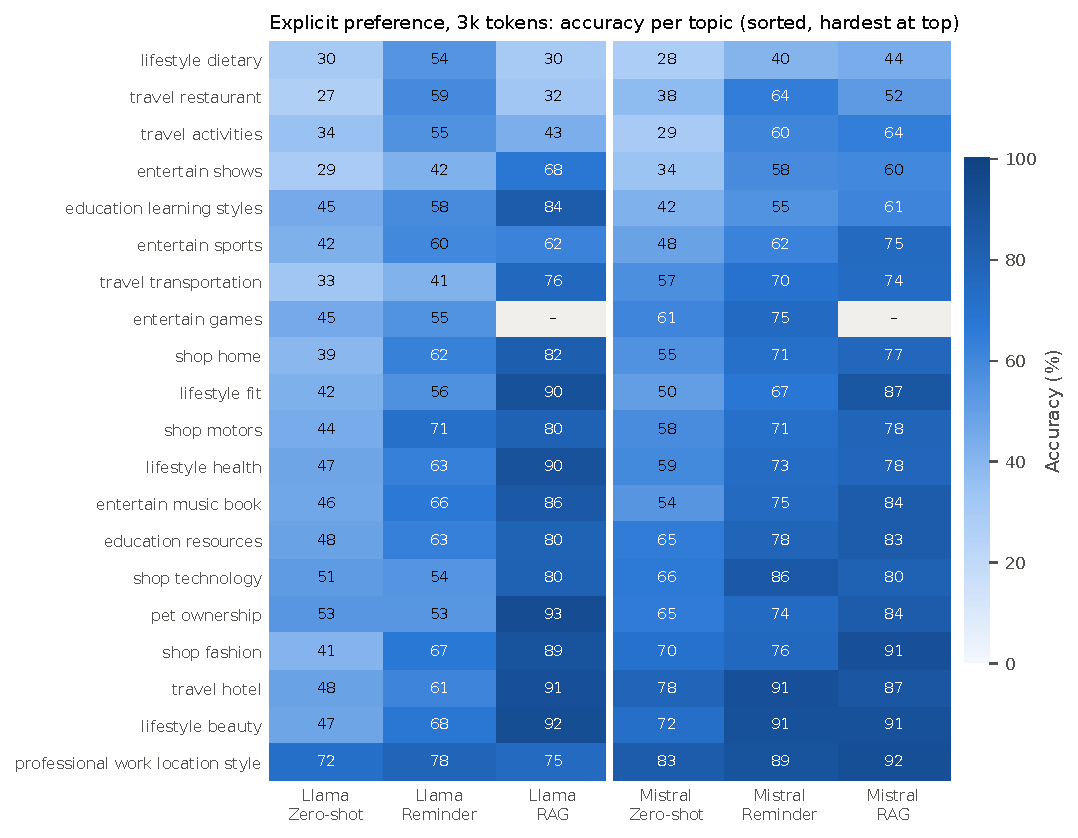
\includegraphics[width=0.78\linewidth]{fig_topic_heatmap.pdf}
\caption{Per-topic accuracy at 3k (explicit preference), sorted from hardest (top) to easiest.}
\label{fig:heatmap}
\end{figure}

%===============================================================================
\section{Deviations from the paper and threats to validity}

\begin{itemize}
  \item \textbf{Serving stack.} The models use 8-bit weights served by llama.cpp instead of full precision on Bedrock, and Mistral also uses an 8-bit KV cache.
        Small numerical differences can flip near-tie answers under greedy decoding.
  \item \textbf{Prompt hygiene.} There are two whitespace / start-token normalisations (Section~\ref{sec:issues}). All prompt \emph{text} is identical to the
        original code.
  \item \textbf{Option shuffling} uses a per-question seed instead of one global random stream. It is still random, but identical
        across methods and lengths, which makes method comparisons paired and runs resumable.
  \item \textbf{RAG coverage} is 19 topics for explicit preferences and 973/1{,}000 questions for implicit ones, because of defects in the released data.
  \item \textbf{Single run per cell.} Greedy decoding makes each run deterministic, but no confidence intervals are reported yet.
        With $\approx$1{,}000 questions per cell, a binomial standard error is at most about 1.6 points per cell.
  \item \textbf{Classification task only.} The generation task needs an LLM judge (Claude 3 Sonnet in the paper) and is not part of
        Phase~1.
\end{itemize}

%===============================================================================
\section{Feasibility review and next steps}\label{sec:next}

\subsection{What the local setup can and cannot do}
\begin{center}\small
\begin{tabular}{p{6.2cm}p{2.0cm}p{6.2cm}}
\toprule
Item & Feasible? & Note \\
\midrule
Classification task, 7--8B models, all methods & Yes & Done in Phase 1 \\
Long regime ($\approx$70 turns) & Yes (Mistral) & Llama-3-8B limited to 8k; Llama-3.1-8B possible without a paper baseline \\
Mixtral-8x7B, 70B models & No & Exceeds 12\,GB GPU + 15\,GB RAM \\
Generation task + four error types & Partially & Needs an LLM judge: an API model on a small subset, or a local judge (not comparable to the paper) \\
Proprietary model (gpt-4o-mini) & Budget-dependent & Planned on a small subset only \\
Phase 2 classifier training & Yes & Small encoders train in minutes \\
\bottomrule
\end{tabular}
\end{center}

\subsection{Phase 2: preference-detection classifier}
\begin{itemize}
  \item \textbf{Data.} Positives: explicit preference sentences and the preference-revealing user turns of the implicit
        dialogues. Negatives: the LMSYS distractor turns and the non-revealing turns of the implicit dialogues. LLM-generated pseudo-labels will add
        variety, as proposed.
  \item \textbf{No leakage.} Phase~3 is evaluated on PrefEval itself, so the classifier will be trained on a \emph{topic-level}
        split (as in the paper's own fine-tuning experiment, 80/20 by topic), and Phase~3 will be reported on the held-out topics. The split
        file will be shared between Phase~2 and Phase~3.
  \item \textbf{Models and metrics.} DistilBERT, ModernBERT and MiniLM. I will report loss curves, held-out accuracy, and precision / recall /
        confusion matrix per preference form, plus per-turn latency vs.\ an LLM-prompted detector.
\end{itemize}

\subsection{Phase 3: full pipeline}
\begin{itemize}
  \item The classifier flags preference turns into a memory list. At query time the memory and the top-$k$ exchanges from a modern encoder
        (bge-base / e5-base, replacing SimCSE) are combined into the prompt.
  \item Evaluation reuses the Phase~1 runner, prompts, parser and settings guard, so the new method and the baselines run under identical
        conditions on both models, both preference forms and all context lengths, including Mistral's long regime.
  \item Targets suggested by Phase~1: the drop from 0.2k to 3k (e.g.\ Llama zero-shot 94 $\rightarrow$ 43), the position-prior
        collapse at long context, and RAG refusals caused by retrieved distractors.
  \item Optional additions if time permits: CoT and Self-Critic for Mistral at 10k--23k (about 20--25\,h), a full-precision KV-cache control
        for the Mistral RAG gap, and a small generation-task sanity check with an LLM judge.
\end{itemize}

%===============================================================================
\section{Conclusion}
Phase~1 is complete. The PrefEval classification benchmark now runs fully on local hardware with the original prompts. It was
evaluated on two of the paper's models, five methods, two preference forms and six context lengths (\nQuestions{} questions),
and every result, setting and run is recorded and reproducible. The paper's main findings reproduce: preference following degrades
quickly with context, Reminder and RAG are the strongest baselines, implicit preferences are harder, and self-critique is
unreliable for classification. Most absolute numbers are within a few points of the paper, and the largest gaps have identified or
plausible causes. Phase~1 also provides concrete targets for the proposed classifier-plus-memory pipeline.

%===============================================================================
\begin{thebibliography}{9}\small
\bibitem{prefeval} S.~Zhao, M.~Hong, Y.~Liu, D.~Hazarika, K.~Lin.
  \emph{Do LLMs Recognize Your Preferences? Evaluating Personalized Preference Following in LLMs.} ICLR 2025. arXiv:2502.09597.
\bibitem{lmsys} L.~Zheng et al. \emph{LMSYS-Chat-1M: A Large-Scale Real-World LLM Conversation Dataset.} ICLR 2024.
\bibitem{simcse} T.~Gao, X.~Yao, D.~Chen. \emph{SimCSE: Simple Contrastive Learning of Sentence Embeddings.} EMNLP 2021.
\bibitem{huang} J.~Huang et al. \emph{Large Language Models Cannot Self-Correct Reasoning Yet.} ICLR 2024.
\bibitem{llama3} Meta AI. \emph{The Llama 3 Herd of Models.} arXiv:2407.21783, 2024.
\bibitem{mistral} A.~Q.~Jiang et al. \emph{Mistral 7B.} arXiv:2310.06825, 2023.
\bibitem{ollama} Ollama (v0.34.0) and llama.cpp, \url{https://ollama.com}, \url{https://github.com/ggml-org/llama.cpp}.
\end{thebibliography}

\appendix
\section{Reproducing the results}
The code is in the project fork, branch \nolinkurl{phase1-local-ollama}. The documentation is in \nolinkurl{docs/PHASE1.md}, the
configs are in \nolinkurl{configs/phase1/}, and the results and run manifest are in \nolinkurl{results/phase1/}.
\begin{verbatim}
conda create -n prefeval python=3.11 && conda activate prefeval
pip install -r requirements-phase1.txt
ollama pull llama3:8b-instruct-q8_0
# run (resumable) one experiment tier
python -m phase1.runner run --config configs/phase1/tierA.yaml
python -m phase1.aggregate       # tables + plots
python report/make_assets.py     # this report's figures
\end{verbatim}
Model digests: Llama \texttt{1b8e49ce\dots}, Mistral \texttt{3f321fd2\dots}
(full values in \nolinkurl{results/phase1/run_manifest.jsonl}). Ollama 0.34.0 was used for all runs.

\section{Use of AI assistance}
Claude (Anthropic) was used as a coding and writing assistant: building the local inference pipeline, diagnosing the issues in
Section~\ref{sec:issues}, generating figures, and drafting this report. All experiments were run on my machine, every number
comes directly from the logged results through a script (\texttt{report/make\_assets.py}), and the project direction, decisions
and interpretation are my own.

\end{document}
